\documentclass[border=4pt]{standalone}
\usepackage{tikz}
\usetikzlibrary{arrows,positioning}
\begin{document}
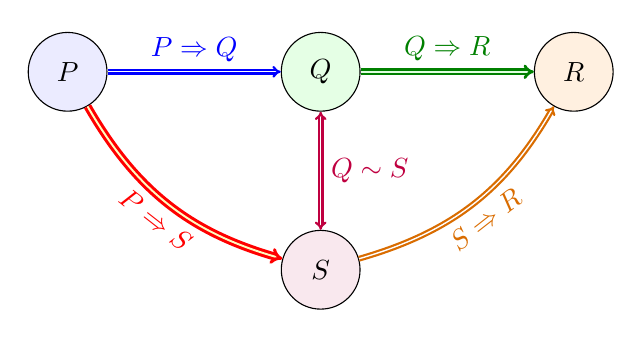
\begin{tikzpicture}[
  node distance=1.5cm and 2.2cm,
  proposition/.style={draw,circle,minimum size=10mm,inner sep=1pt}
]
  \node[proposition,fill=blue!8] (p) {$P$};
  \node[proposition,fill=green!10,right=of p] (q) {$Q$};
  \node[proposition,fill=orange!12,right=of q] (r) {$R$};
  \node[proposition,fill=purple!9,below=of q] (s) {$S$};

  \draw[blue,double=white,line width=.8pt,double distance=.5pt,-implies]
    (p) -- node[above] {$P\Rightarrow Q$} (q);
  \draw[green!50!black,double=green!12,line width=1pt,double distance=.6pt,-implies]
    (q) -- node[above] {$Q\Rightarrow R$} (r);
  \draw[purple,double=white,line width=.8pt,double distance=.5pt,implies-implies]
    (q) -- node[right] {$Q\sim S$} (s);
  \draw[red,double=yellow!25,line width=1.1pt,double distance=.7pt,-implies]
    (p) to[bend right=22] node[below,sloped] {$P\Rightarrow S$} (s);
  \draw[orange!85!black,double=white,line width=.8pt,double distance=.5pt,-implies]
    (s) to[bend right=22] node[below,sloped] {$S\Rightarrow R$} (r);
\end{tikzpicture}
\end{document}
